
%----------------------------------------------------------------------------------------
%	PACKAGES AND OTHER DOCUMENT CONFIGURATIONS
%----------------------------------------------------------------------------------------

\documentclass[12pt]{article}

\usepackage{graphicx}
\usepackage{epsfig}
\usepackage{psfrag}
%\usepackage{subfigure}
%\usepackage{subfig}
%\usepackage{tabularx}
\usepackage{subfigmat}
\usepackage{subeqnarray}
\usepackage[colorlinks]{hyperref}
\usepackage{amsmath,amsfonts,amsfonts,amsthm}
\usepackage{xcolor,colortbl}
\usepackage[mathscr]{euscript}
\usepackage{algorithm2e}
\usepackage{siunitx}
\usepackage{rotating}
\usepackage{bm}
\setcounter{secnumdepth}{3}
\usepackage[version=3]{mhchem} 
\usepackage{graphicx}
\usepackage{fancyvrb}
\usepackage[top=1in, bottom=1in, left=1in, right=1in]{geometry}
\graphicspath{{../Figures/}}
\usepackage{color}
\usepackage{pdfpages}
\usepackage{enumitem}
\usepackage{bbm}

\newcommand\alignedbox[2]{
	% Argument #1 = before & if there were no box (lhs)
	% Argument #2 = after & if there were no box (rhs)
	&  % Alignment sign of the line
	{
		\settowidth\dlf{$\displaystyle #1$}  
		% The width of \dlf is the width of the lhs, with a displaystyle font
		\addtolength\dlf{\fboxsep+\fboxrule}  
		% Add to it the distance to the box, and the width of the line of the box
		\hspace{-\dlf}  
		% Move everything dlf units to the left, so that & #1 #2 is aligned under #1 & #2
		\boxed{#1 #2}
		% Put a box around lhs and rhs
	}
}
%----------------------------------------------------------------------------------------
%	ABBREVIATIONS SECTIONS
%----------------------------------------------------------------------------------------
 \newcommand{\dod}{\mathrm{C}_{12}\mathrm{H}_{26}}
 \newcommand{\nit}{\mathrm{N}_{2}}
 \newcommand{\ox}{\mathrm{O}_{2}}
 \newcommand{\wat}{\mathrm{H}_{2}\mathrm{O}}
 \newcommand{\cardiox}{\mathrm{C}\mathrm{O}_{2}}

\begin{document}
\input{abbrevs}
\begin{titlepage}

\newcommand{\ddz}[1]{\frac{\mathrm{d} #1}{\mathrm{d} z}}
\newcommand{\HRule}{\rule{\linewidth}{0.5mm}} % Defines a new command for the horizontal lines, change thickness here

\center % Center everything on the page
 

 
%----------------------------------------------------------------------------------------
%	HEADING SECTIONS
%----------------------------------------------------------------------------------------


%\textsc{\Large STANFORD UNIVERSITY}\\[1.5cm] % Name of your university/college

%----------------------------------------------------------------------------------------
%	TITLE SECTION
%----------------------------------------------------------------------------------------

\HRule \\[1 cm]
{ \huge \bfseries Problem Set 2 Solutions}\\[0.4cm] % Title of your document
\HRule \\[2cm]
 
%----------------------------------------------------------------------------------------
%	AUTHOR SECTION
%----------------------------------------------------------------------------------------

\Large  \textsc{Matthias Ihme}\\[2cm] % Your name
\textsc{\large ME 257/357: Propulsion System and Gas-Turbine Analysis}\\[2cm] % Major heading such as course name

%----------------------------------------------------------------------------------------
%	LOGO SECTION
%----------------------------------------------------------------------------------------
\includegraphics[width=50mm]{stanford_seal.png}\\[2cm] % Include a department/university logo - this will require the graphicx package
%----------------------------------------------------------------------------------------
%----------------------------------------------------------------------------------------
%	DATE SECTION
%----------------------------------------------------------------------------------------
{\large Spring 2018}%\\[3cm] % Date, change the \today to a set date if you want to be precise

\vfill % Fill the rest of the page with whitespace

\end{titlepage}

%----------------------------------------------------------------------------------------
%	BODY SECTION
%----------------------------------------------------------------------------------------

%%%%%%%%%%%%%%%%%%%%%%%%%%%%%%%%%%%%%%%%%%%%%%%%%%%%%%%%%%%%%%%%%%%%%%%%%%%%%%%%  
\section{Problem 1: Equilibrium Combustion (30 pts)}
	\subsection{Combustion Mixture Composition (10 pts)}
	\begin{enumerate}[label=(\alph*)]
		\item (5 pts) \\
			\textbf{Stoichiometric Case} ($\phi = 1$): 
			\begin{equation}
				\boxed{\dod+37/2(\ox+3.76\nit)\rightarrow 12\cardiox+13\wat+37/2(3.76\nit)}
			\end{equation}
			\textbf{Fuel-Lean Case} ($\phi < 1$): 
			\begin{equation}
			\boxed{\phi\dod+37/2(\ox+3.76\nit)\rightarrow 12\phi\cardiox+13\phi\wat+37/2(3.76\nit)+\frac{37}{2}(1-\phi)\ox}
			\end{equation}
			\textbf{Fuel-.Rich Case} ($\phi > 1$): 
			\begin{equation}
			\boxed{\phi\dod+37/2(\ox+3.76\nit)\rightarrow 12\cardiox+13\wat+37/2(3.76\nit)+(\phi-1)\dod}
			\end{equation}
		\item (5 pts) \\
			Figure~\ref{FIG_1pt1b} shows the species product mass fractions against the equivalence ratio. Note that the species product mass fraction of the $i^{\mathrm{th}}$ species, $Y_i$, is found by
			\begin{equation}
				Y_i=\frac{\nu_i^{\prime\prime}W_i}{\sum_j \nu_j^{\prime\prime}W_i}\ ,
			\end{equation}
			where $\nu_i^{\prime\prime}$ is the number of moles in the products of the reaction for species $i$, and $W_i$ is the molecular weight of the $i^{\mathrm{th}}$ species.
			\begin{figure}[!t!]
				\begin{center}
					\includegraphics[width=120mm]{problem1pt1b.pdf}
					\caption{\label{FIG_1pt1b} Plots of the mass fractions of $\wat$ and $\cardiox$ against the equivalence ratio.}
				\end{center}
			\end{figure}
	\end{enumerate}
%================================================================================
	\subsection{Adiabatic Flame Temperature (20 pts)}
	\begin{enumerate}[label=(\alph*)]
		\item (5 pts)
		The heat of combustion is given by
			\begin{equation}
				\begin{aligned}
					H_\mathrm{c}&=-H_\mathrm{r}^0\ , \\
					&=-\left[\sum_i(\nu_i^{\prime\prime}-\nu_i^{\prime})\Delta H_{\mathrm{f},i}W_i\right]\\
					&=-12\min(1,\phi)\Delta H_{\mathrm{f},\cardiox}W_\cardiox-13\min(1,\phi)\Delta H_{\mathrm{f},\wat}W_{\wat}\\
					&+[\phi-\max(0,\phi-1)] H_{\mathrm{f},\dod}W_{\dod}\\
					&=\min(1,\phi)\left(\Delta H_{\mathrm{f},\dod}W_{\dod}-12\Delta H_{\mathrm{f},\cardiox}W_{\cardiox}-13\Delta H_{\mathrm{f},\wat}W_{\wat}\right) \\
					&=\boxed{7.57\min(1,\phi)\ \mathrm{MJ}}\ ,
				\end{aligned}
			\end{equation}
		where the values from Table 1 are substituted between lines 5 and 6. Note, that a unit conversion took place between lines 4 and 5 to ensure that $\Delta H_{\mathrm{f},i}=\mathrm{[J/g]}$, and the references species are left out since they do not contribute to the heat of combustion. 
		
		Hence, it is shown that the heat of combustion is constant for lean conditions, and depends on the equivalence ratio for the rich conditions. Physically, for $\phi>1$, the fuel is burned and does not release any additional energy
		
		The LHV is given by the stoichiometric conditon: $\boxed{\mathrm{LHV=7.57\ [MJ/mol]}}$.
		
		Additionally, it is shown that since $H_\mathrm{c}>0$, the reaction is $\boxed{\mathrm{exothermic}}$.	
		\item (5 pts)
			From conservation of energy, the adiabatic flame temperature, $T_\mathrm{ad}$ is found by
			\begin{equation}
				\begin{aligned}
					H_\mathrm{c}&=C_{p,\mathrm{prod}}(T_\mathrm{ad}-T_\mathrm{ref})-C_{p,\mathrm{reac}}(T_\mathrm{reac}-T_\mathrm{ref})\\
					\implies T_\mathrm{ad}&=\boxed{T_\mathrm{ref}+\frac{H_\mathrm{c}+C_{p,\mathrm{reac}}(T_\mathrm{reac}-T_\mathrm{ref})}{C_{p,\mathrm{prod}}}}
				\end{aligned}
			\end{equation}
			The reference temperature is known to be 298 K. $H_\mathrm{c}$ is given by the results of part a. The specific heats are given by \\
			\begin{subeqnarray}
				C_{p,\mathrm{reac}} & = & \sum_i c_{p,i}\nu_i^{\prime\prime}W_i\\
				C_{p,\mathrm{prod}} & = & \sum_i c_{p,i}\nu_i^{\prime}W_i
			\end{subeqnarray}
			where the stoiciometric coefficients are those given in Problem 1.1a. 
			
		\item (5 pts)
			See solution code for cantera implementation.
		\item (5 pts)	
			A comparison of the calorically perfect gas model with an equilibrium solver (i.e., cantera) is shown in Fig.~\ref{FIG_1pt2}. The calorically perfect gas model results in lower adiabatic flame temperatures for all equivalence ratios; much of the discrepancy can be attributed to $c_p$ increasing with $T$, which is not captured by the calorically perfect model. However at lean conditions, the two models align quite well; at these conditions, the composition of the product gas is well-described without the effect of additional products not accounted for in our analysis (e.g., carbon monoxide).
			\begin{figure}[!t!]
				\begin{center}
					\includegraphics[width=120mm]{problem1pt2.pdf}
					\caption{\label{FIG_1pt2} Adiabatic flame temperatures predicted for two models}
				\end{center}
			\end{figure}
	\end{enumerate}
%%%%%%%%%%%%%%%%%%%%%%%%%%%%%%%%%%%%%%%%%%%%%%%%%%%%%%%%%%%%%%%%%%%%%%%%%%%%%%%%
\section{Problem 2: Gas-Turbine Combustor Design (90 pts)}
	\subsection{Combustor Inlet Conditions (15 pts)}
		\begin{enumerate}[label=(\arabic*)]
			\item (5 pts)
				The overall-fuel air ratio is given by
				\begin{equation}
					f = \frac{T_{04}/T_{03}-1}{\mathrm{LHV}/(c_pT_{03})-T_{04}/T_{03}}\ .
				\end{equation}
				From before $\mathrm{LHV}=7.57\ \mathrm{MJ/mol}=44.5\ \mathrm{kJ/kg}$ (note that heating values are given per unit of the fuel). Additionally, $T_{04}-1600$ K and $c_p=$ 1005 [J/kg.K]. Now for an ideal turbojet, $T_{03}$ is given by
				\begin{equation}
					T_{03}=T_0\tau_{r}\tau_{c}\ .
				\end{equation}
				where $\tau_r=1+(\gamma-1)M_0^2/2=1.10$ and $\tau_c=\pi_c^{(\gamma-1)/\gamma}=2.48$. Note, $\gamma=cp/(cp-R)=1.4$. Hence, $T_{03}=585$. This gives an overall fuel-air ratio of $\boxed{f=0.0238}$
			\item (5 pts)
				The overall-fuel air ratio is as before. The equivalence ratio is given by 
				\begin{equation}
					\begin{aligned}
						\phi&=\frac{f}{f_\mathrm{st}}\\
							&=\frac{f}{m_{\dod,\mathrm{st}}/\left(m_{\ox,\mathrm{st}}+m_{\nit,\mathrm{st}}\right)}\\
							&=\frac{0.0238}{170/(592+1948)}\\
							&=\boxed{0.355}
					\end{aligned}
				\end{equation}
			\item (5 pts)
				The stagnation density at the inlet of the combustor is given by the ideal gas law: $\rho_{03}=p_{03}/(RT_{03})$. In a similar manner to the temperature, the pressure is given by $p_{03}=p_0\pi_r\pi_c$, where $\pi_r=\tau_r^{\gamma/(\gamma-1)}=1.39$ and $\pi_c$ is given as 24. $p_0$ is taken to be the pressure at 43 kft, which is 0.162 bar. Hence, $p_{03}=5.40$ bar $\implies \boxed{\rho_{03}=3.22}$. 
		\end{enumerate}
%================================================================================
	\subsection{Combustor Area (10 pts)}
	\begin{enumerate}[label=(\alph*)]
		\item (5 pts)
			The geometry is shown in Fig.~\ref{FIG_2pt2}. The radius of the can combustor is given by $R_\mathrm{c}=(R_\mathrm{o}-R_\mathrm{i})/2$. Furthermore, the angle, $\theta$ is found from 
			\begin{equation}
				\theta = \arcsin\left(\frac{R_\mathrm{c}}{R_\mathrm{i}+R_\mathrm{c}}\right)
			\end{equation} 
			Hence, the number of can combustors is given by
			\begin{equation}
				n_\mathrm{comb} =\boxed{\left\lfloor{\frac{\pi}{\theta}}\right\rfloor}
			\end{equation}
			where $\lfloor x\rfloor$ denotes the floor operation on the variable $x$. 
			\begin{figure}[!t!]
				\begin{center}
					\includegraphics[width=120mm]{problem2pt2.pdf}
					\caption{\label{FIG_2pt2} Cartoon of the configuration of the combustors in the cross-sections.}
				\end{center}
			\end{figure}
		\item (5 pts)
			$A_c=\pi R_\mathrm{c}^2=3.14\times0.15^2=\boxed{0.0177\ \mathrm{m^2}}$
	\end{enumerate}
%================================================================================
\subsection{Combustor Length (65 pts)}
	\begin{enumerate}[label=(\alph*)]
		\item (5 pts)
			The overall length of the combustor, $L$, is given by
			\begin{equation}
				L = \sum_{s\in S}U_s\tau_s
			\end{equation} 
			where $S=\{\mathrm{mix,evap,dil,srz}\}$.
		\item \textit{Evaporation and mixing}(25 pts)
			\begin{enumerate}[label=(\roman*)]
				\item (5 pts)
					The velocity of the air is given by
					\begin{equation}
						\begin{aligned}
							U_{a1}&=\frac{\dot{m}_{a1}}{\rho_{a1}A_{a1}}\\
							&=\frac{\dot{m}_{a1}}{\rho_{03}A_{a1}}\\
							&=\frac{\dot{m}_{a1}+\dot{m}_{a2}}{(1+\beta_c)\rho_{03}A_{a1}}\\
							&=\frac{\dot{m}_{a}}{(1+\beta_c)n_\mathrm{comb}\rho_{03}A_{a1}}\\
							&=\frac{\dot{m}_{a}}{(1+\beta_c)n_\mathrm{comb}\rho_{03}(A_{c}-A_f)}\\
							&=\boxed{\frac{\dot{m}_{a}}{(1+\beta_c)n_\mathrm{comb}\rho_{03}A_c(1-\beta_\mathrm{mix})}}\\
						\end{aligned}
					\end{equation}
				\item (5 pts)
					The fuel air ratio at the inlet is given by
					\begin{equation}
						\begin{aligned}
							f_\mathrm{mix}&=\frac{\dot{m}_F/n_\mathrm{comb}}{\dot{m}_{a1}}\\
							&=\frac{\dot{m}_F(1+\beta_\mathrm{c})}{\dot{m}_{a}}\\
							&=\boxed{(1+\beta_\mathrm{c})f}\ .
						\end{aligned}
					\end{equation} 
					Since $f\propto \phi\implies \boxed{\phi_\mathrm{mix}=(1+\beta_\mathrm{c})\phi}$.
				\item (5 pts)
					The change in mass of a spherical droplet is given by
					\begin{equation}
						\begin{aligned}
							\frac{\d m_\mathrm{drop}}{\d t}&=-\dot{m}_\mathrm{evap}\\
							&=2\pi D\frac{\lambda_\mathrm{g}\log(1+\mathcal{B})}{c_{p\mathrm{g}}}\\
							&=-\frac{\pi D\rho_F}{4}\beta
						\end{aligned}
					\end{equation} 
					Now, since
					\begin{equation}
						\begin{aligned}
							m_\mathrm{drop}&=\rho_F\left(\frac{\pi D^3}{6}\right)\\
							\implies \frac{\d m_\mathrm{drop}}{\d t}&=\rho_F\left(\frac{\pi}{6}\right)\frac{\d}{\d t}\left[(D^2)^{\frac{3}{2}}\right]\\
							&=\frac{\pi D\rho_F}{4}\frac{\d(D^2)}{\d t}\ ,
						\end{aligned}
					\end{equation} 
					this gives through substitution
					\begin{equation}
						\begin{aligned}
							\frac{\pi D\rho_F}{4}\frac{\d(D^2)}{\d t}&=-\frac{\pi D\rho_F}{4}\beta\\ 
							\implies \frac{\d(D^2)}{\d t}&=-\beta \\
							\implies \int_{D_0^2}^{D^2}\d(D^{\prime 2})&=-\beta\int_{0}^{t}\d t^\prime\\
							\implies D^2-D_0^2&=-\beta t\\
							\implies \frac{D}{D_0}&=\sqrt{1-\frac{t}{D_0^2/\beta}} \\
							&=\boxed{\sqrt{1-\frac{t}{\tau_\mathrm{evap}}}}\\
						\end{aligned}
					\end{equation} 
				\item (Bonus 5 pts)
					The Rossin-Rammler distribution for $\alpha=2$ is given by
					\begin{equation}
						\begin{aligned}
							F(D_0;D_\sigma)=1-\exp\left[-\left(\frac{D_0}{D_\sigma}\right)^{2}\right]\ .
						\end{aligned}
					\end{equation} 
					Define $\Delta=(D_0/D_\sigma)^2$. The probability density function of the Rossin-Rammler distribution with respect to $\Delta$ is given by
					\begin{equation}
						\begin{aligned}
							f(\Delta)&=\frac{\d F}{\d \Delta} \\
							&=\exp(-\Delta)\ .
						\end{aligned}
					\end{equation}
					From part ii, $\tau_\mathrm{evap}=D_0^2/\beta=D_\mathrm{\sigma}^2\Delta/\beta$. Therefore, the mean evaporation time of a droplet in a spray, $\mathrm{E}(\tau_\mathrm{evap})$, is given by
					\begin{equation}
						\begin{aligned}
							\mathrm{E}(\tau_\mathrm{evap})&=\frac{D_\sigma^2}{\beta}\int_0^\infty \Delta\exp(-\Delta)\d \Delta \\
							&=\frac{D_\sigma^2}{\beta}\left(\left . -\frac{\Delta}{\exp(\Delta)}\right|_0^\infty+\int_0^{\infty}\exp(-\Delta)\d\Delta\right)\\
							&=\frac{D_\sigma^2}{\beta}\int_0^{\infty}\exp(-\Delta)\d\Delta\\
							&=\boxed{\frac{D_\sigma^2}{\beta}}\ .
						\end{aligned}
					\end{equation}
					Hence, the mean evaporation time in a spray is simply the $D^2$ law applied to the Sauter Mean Diameter, $D_\sigma$, for $\alpha=2$.
				\item (5 Pts)
					The length of the evaporation is given by $L_\mathrm{evap}=\boxed{\tau_\mathrm{evap}U_\mathrm{e}}$
			\end{enumerate}
		\item \textit{Flame} (5 pts)
			\begin{enumerate}[label=(\roman*)]
				\item (5 pts) 
				Conservation of mass gives 
				\begin{equation}
					\begin{aligned}
						\rho_\mathrm{evap}U_\mathrm{e}A_c&=\rho_\mathrm{flame}U_\mathrm{flame}A_c\\
						\implies U_\mathrm{flame}&=U_\mathrm{e}\left(\frac{\rho_\mathrm{evap}}{\rho_\mathrm{flame}}\right)
					\end{aligned}
				\end{equation}
				Furthermore, Using the ideal gas law and assuming negligible change in composition ($R_\mathrm{evap}\approx R_\mathrm{flame}$) and an isobaric process yields
				\begin{equation}
					\begin{aligned}
						\rho_\mathrm{flame}T_\mathrm{flame}&=\rho_\mathrm{evap}T_\mathrm{evap}\\
						\implies \frac{\rho_\mathrm{evap}}{\rho_\mathrm{flame}}&=\frac{T_\mathrm{flame}}{T_\mathrm{evap}}\ .
					\end{aligned}
				\end{equation}
				Hence,
				\begin{equation}
					\begin{aligned} U_\mathrm{flame}&=\boxed{U_\mathrm{e}\left(\frac{T_\mathrm{flame}}{T_\mathrm{evap}}\right)}
					\end{aligned}
				\end{equation}
				Since $T_\mathrm{flame}>T_\mathrm{evap}$, the speed $\boxed{\mathrm{increases}}$.
			\end{enumerate}
		\item \textit{Dilution} (20 pts)
			\begin{enumerate}[label=(\roman*)]
				\item (5 pts)
					Conservation of mass can be used to relate the mass flow of the rerouted air to the velocity of the dilution jet:
					\begin{equation}
						\begin{aligned} 				
							\dot{m}_{a2}&=n_\mathrm{dil}\rho_\mathrm{jet}U_\mathrm{jet}A_{\mathrm{jet}}\\
							&=n_\mathrm{dil}\rho_\mathrm{03}U_\mathrm{jet}A_{\mathrm{jet}}\\
							&=n_\mathrm{dil}\rho_\mathrm{03}U_\mathrm{jet}\frac{\pi d_\mathrm{dil}^2}{4}\\
							\implies U_\mathrm{jet}&=\frac{4\dot{m}_{a2}}{\pi n_\mathrm{dil}\rho_{03}d_\mathrm{dil}^2}\\
							&=\frac{4\dot{m}_{a1}\beta_c}{\pi n_\mathrm{dil}\rho_{03}d_\mathrm{dil}^2}\\
							&=\boxed{\frac{4\dot{m}_{a}\beta_c}{\pi(1+\beta_c)n_\mathrm{comb} n_\mathrm{dil}\rho_{03}d_\mathrm{dil}^2}}
						\end{aligned}
					\end{equation}
				\item (5 pts)
					The concentration of the jet in the fully mixed state is given by 
					\begin{equation}
						\begin{aligned} 				
							c_\mathrm{f}&=\frac{n_\mathrm{comb}\dot{m}_{a2}}{\dot{m}_{a}+\dot{m}_\mathrm{F}}\\
							&=\frac{n_\mathrm{comb}\dot{m}_{a2}}{\dot{m}_{a}(1+f)}\\
							&=\frac{\dot{m}_{a2}}{(\dot{m}_{a1}+\dot{m}_{a2})(1+f)}\\
							&=\boxed{\frac{\beta_c}{(1+\beta_c)(1+f)}}
						\end{aligned}
					\end{equation}
				\item (5 pts)
					The dilution length, $L_\mathrm{dil}$ is found by
					\begin{equation}
						\begin{aligned}
							\frac{c_\mathrm{f}}{C_\mathrm{dil}}&=\left(\frac{L_\mathrm{dil}}{\xi d_\mathrm{dil}}\right)^{-2/3} \\
							\implies L_\mathrm{dil}&=\boxed{\left(\frac{c_\mathrm{f}}{C_\mathrm{dil}}\right)^{-3/2}\xi d_\mathrm{dil}}
						\end{aligned}
					\end{equation}
				\item (5 pts)
					From mass conservation
					\begin{equation}
						\begin{aligned}
							\rho_\mathrm{dil}U_\mathrm{dil}A_c=\frac{\dot{m}_{a}(1+f)}{n_\mathrm{comb}}\\
							\implies U_\mathrm{dil}=\boxed{\frac{\dot{m}_{a}(1+f)}{n_\mathrm{comb}\rho_\mathrm{dil}A_c}}
						\end{aligned}
					\end{equation}
					Additionally, for adiabatic, isobaric mixing with constant $c_p$ and $R$: 
					\begin{equation}
						\begin{aligned}
							\dot{m}_{a}(1+f)h_\mathrm{dil}&=(n_\mathrm{comb}\dot{m}_{a1}+\dot{m}_F)h_\mathrm{flame}+n_\mathrm{comb}\dot{m}_{a2}h_{03}\\
							\implies \dot{m}_{a}(1+f)T_\mathrm{dil}&=(n_\mathrm{comb}\dot{m}_{a1}+\dot{m}_F)T_\mathrm{flame}+n_\mathrm{comb}\dot{m}_{a2}T_{03}\\
							\implies T_\mathrm{dil}&=\frac{(n_\mathrm{comb}\dot{m}_{a1}/\dot{m}_a+f)T_\mathrm{flame}+n_\mathrm{comb}\dot{m}_{a2}/\dot{m}_a T_{03}}{(1+f)}\\
							&=\frac{[1+(1+\beta_c)f]T_\mathrm{flame}+\beta_c T_{03}}{(1+\beta_c)(1+f)}\\
							&=T_{03}\frac{[1+(1+\beta_c)f]T_\mathrm{flame}/T_{03}+\beta_c }{(1+\beta_c)(1+f)}\\
							\implies \rho_\mathrm{dil}&=\boxed{\frac{\rho_{03}(1+\beta_c)(1+f)}{[1+(1+\beta_c)f]T_\mathrm{flame}/T_{03}+\beta_c }}
						\end{aligned}
					\end{equation}
			\end{enumerate}
		\item \textit{Secondary Reaction Zone} (10 pts)
			\begin{enumerate}[label=(\roman*)]
				\item (5 pts)
					If half of the inlet fuel and air is combusted, then 
					\begin{equation}
						\begin{aligned}
							\phi_\mathrm{srz} &= f_\mathrm{st}^{-1}\left(\frac{\dot{m}_{F,\mathrm{srz}}}{\dot{m}_{a,\mathrm{srz}}}\right)\\ 
							&=f_\mathrm{st}^{-1}\left(\frac{\dot{m}_{F}}{2\dot{m}_{a,\mathrm{srz}}}\right)\\ 
							&=f_\mathrm{st}^{-1}\left[\frac{\dot{m}_{F}}{2(n_\mathrm{comb}\dot{m}_{a2}+n_\mathrm{comb}\dot{m}_{a1}/2)}\right]\\ 
							&=f_\mathrm{st}^{-1}\left[\frac{\dot{m}_{F}}{\dot{m}_a\left(\frac{2\beta_c}{1+\beta_c}+\frac{1}{1+\beta_c}\right)}\right]\\ 
							&=\boxed{\phi\left(\frac{1+\beta_c}{1+2\beta_c}\right)}\\ 
						\end{aligned}
					\end{equation}
					Note that for $\beta_c>>1,\ \phi_\mathrm{srz}\approx\phi/2$. 
				\item (5 pts)
					The length of the secondary reaction zone is given by $L_\mathrm{srz}=U_\mathrm{srz}\tau_\mathrm{srz}=\boxed{U_\mathrm{dil}\tau_\mathrm{srz}}$
			\end{enumerate}
	\end{enumerate}
%%%%%%%%%%%%%%%%%%%%%%%%%%%%%%%%%%%%%%%%%%%%%%%%%%%%%%%%%%%%%%%%%%%%%%%%%%%%%%%%
\section{Problem 3: Model Analysis (10 pts)}
	A plot showing the lengths within the combustor is shown in Fig.~\ref{FIG_3}.
	\begin{figure}[!t!]
		\begin{center}
			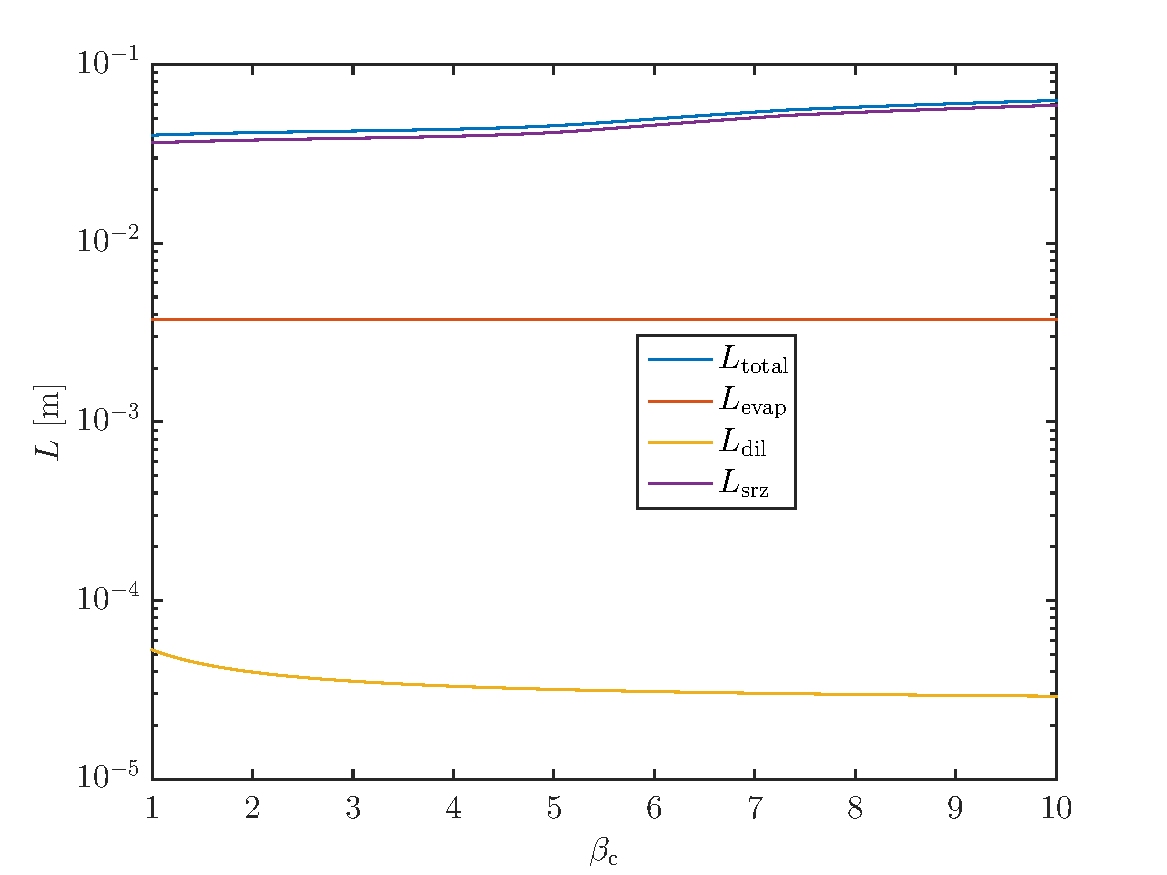
\includegraphics[width=120mm]{problem3.pdf}
			\caption{\label{FIG_3} Length scales for the prescribed parameters, and modeling conditions}
		\end{center}
	\end{figure}
%%%%%%%%%%%%%%%%%%%%%%%%%%%%%%%%%%%%%%%%%%%%%%%%%%%%%%%%%%%%%%%%%%%%%%%%%%%%%%%%
\end{document}